\documentclass[12pt,a4paper]{article}
\usepackage[a4paper,total={160mm,250mm}]{geometry}
\usepackage[utf8]{inputenc}
\usepackage[ruled,vlined]{algorithm2e}
\usepackage{amsmath}
\usepackage{amsthm}
\usepackage{amsfonts}
\usepackage{amssymb}
\usepackage{amscd}
\usepackage{array}
\usepackage{caption}
\usepackage{dirtree}
\usepackage{enumitem}
\usepackage{graphicx}
\usepackage{hyperref}
\usepackage{listings}
\usepackage{mathtools}
\usepackage{ngerman}
\usepackage{subcaption}
\usepackage{tcolorbox}
\usepackage{tikz}
\usepackage{xcolor}

\definecolor{shade}{gray}{.5}

\renewcommand{\thesubfigure}{\roman{subfigure}}

\theoremstyle{definition}
\newtheorem{aufgabe}{Aufgabe}

\theoremstyle{definition}
\newtheorem*{losung*}{Lösung}

\theoremstyle{definition}
\newtheorem*{beispiel*}{Beispiel}

\definecolor{mygreen}{rgb}{0,0.6,0}
\definecolor{mygray}{rgb}{0.5,0.5,0.5}
\definecolor{mymauve}{rgb}{0.58,0,0.82}
\definecolor{lightgray}{rgb}{0.9,0.9,0.9}

\lstset{inputpath=../raytracer}
\lstdefinestyle{python}{
	backgroundcolor=\color{lightgray},   % choose the background color; you must add \usepackage{color} or \usepackage{xcolor}; should come as last argument
	basicstyle=\footnotesize\ttfamily,        % the size of the fonts that are used for the code
	breakatwhitespace=false,         % sets if automatic breaks should only happen at whitespace
	breaklines=true,                 % sets automatic line breaking
	captionpos=b,                    % sets the caption-position to bottom
	commentstyle=\color{mygreen},    % comment style
	deletekeywords={...},            % if you want to delete keywords from the given language
	escapeinside={\\[}{\\]},          % if you want to add LaTeX within your code
	extendedchars=true,              % lets you use non-ASCII characters; for 8-bits encodings only, does not work with UTF-8
	firstnumber=1,                   % start line enumeration with line 1000
	frame=single,	                 % adds a frame around the code
	keepspaces=true,                 % keeps spaces in text, useful for keeping indentation of code (possibly needs columns=flexible)
	keywordstyle=\color{blue},       % keyword style
	language=Python,                 % the language of the code
	literate=%
	    {ä}{{\"a}}1%
		{ö}{{\"o}}1%
		{ü}{{\"u}}1%
		{ß}{{\ss}}1%
		{Ä}{{\"A}}1%
		{Ö}{{\"O}}1%
		{Ü}{{\"U}}1,%
	morekeywords={*,...},            % if you want to add more keywords to the set
	numbers=left,                    % where to put the line-numbers; possible values are (none, left, right)
	numbersep=5pt,                   % how far the line-numbers are from the code
	numberstyle=\tiny\color{mygray}, % the style that is used for the line-numbers
	rulecolor=\color{black},         % if not set, the frame-color may be changed on line-breaks within not-black text (e.g. comments (green here))
	showspaces=false,                % show spaces everywhere adding particular underscores; it overrides 'showstringspaces'
	showstringspaces=false,          % underline spaces within strings only
	showtabs=false,                  % show tabs within strings adding particular underscores
	stepnumber=1,                    % the step between two line-numbers. If it's 1, each line will be numbered
	stringstyle=\color{mymauve},     % string literal style
	tabsize=4,	                     % sets default tabsize to 2 spaces
	title=\lstname,                   % show the filename of files included with \lstinputlisting; also try caption instead of title
	rangeprefix=\#---,
	rangesuffix=---,
	includerangemarker=false
}

%\pagestyle{empty}

\title{Eigengesichter}
\author{Oliver Rietmann}
\date{\today}

\begin{document}
\begin{titlepage}
	{\hspace{-1cm}
\includegraphics[width=0.3\textwidth]{images/ETHlogo}\par}
	\vspace{1cm}
	\begin{center}
	{\scshape Mentorierte Arbeit in Fachdidaktik Mathematik\par}
	\vspace{1cm}
	{\large\bfseries Eigengesichter\par}
	\vspace{1cm}
	{Oliver Rietmann\par}
	\vfill
	\end{center}
	{\bfseries Inhalt\par}
	{In dieser Arbeit wird die Technik der \textit{Eigengesichter} (engl. \textit{eigenfaces}) erklärt. Hierbei handelt es sich um eine eine rudimentäre Methode zur Gesichtserkennung, welche durch Computer automatisiert werden kann. Unter Gesichtserkennung versteht man klassischerweise das (automatisierte) identifizieren einer Person auf einem Foto. Aber auch damit verwandte Aufgaben werden hier besprochen.
	Diese Arbeit führt die Leser durch eine Anleitung zur Implementierung eines solchen Programms in Python. Der Fokus liegt dabei auf der zugrundeliegenden Mathematik dieses Verfahrens. Die dazu verwendeten Unterrichtsmethoden sollen zudem aus didaktischer Sicht beleuchtet werden.\par}
	\vspace{0.5cm}
	{\bfseries Zielpublikum\par}
	{Fortgeschrittene gymnasiale Mittelschüler mit Schwerpunkt Mathematik und Studenten einer mathematischen/technischer Fachrichtung.\par}
	\vspace{0.5cm}
	{\bfseries Voraussetzungen\par}
	{Vertrautheit mit den Grundbegriffen der linearen Algebra (Vektoren, Matrizen, Basis, Linearkombination, Unterräume von $\mathbb R^n$).
	Zudem werden grundlegende Programmierkenntnisse vorausgesetzt.\par}
	\vspace{0.5cm}
	{\bfseries Form\par}
	{Text mit Aufgaben, Lösungen und Lernzielen. Die Python-Codes befinden sich im Anhang. Alternativ können sie online heruntergeladen werden. (Der Link befindet sich in der Arbeit.)\par}
	\vspace{0.5cm}
	{\bfseries Betreuung\par}
	{Christian Rüede\par}
	\vspace{0.5cm}
	{\bfseries Datum\par}
	{\today\par}
\end{titlepage}
%\maketitle
%\tableofcontents
\clearpage
\section*{Einleitung}
Historisch gesehen war die Methode der Eigengesichter das erste durch Computer automatisierbare Verfahren zur Gesichtserkennung.
Das Fundament dazu wurde 1987 durch Sirovich and Kirby entwickelt \cite{SirovichKirby1987}.
In ihrer Arbeit verwendeten Sie bereits den Begriff \textit{eigenpictures}.
Sie zeigten auf, wie man Fotos von Gesichtern geeignet durch Begriffe der linearen Algebra beschreiben kann.
Damit war der Weg frei um die mächtige Maschinerie der Mathematik, insbesondere der linearen Algebra und der Statistik, auf Fotos anzuwenden.
Dies geschah schon kurz darauf, nämlich 1991, durch Turk und Pentland \cite{Turk1991}.
Sie verwendeten bereits den Begriff \textit{eigenfaces} und beschrieben das Verfahren zur Gesichtserkennung, welches auch wir implementieren werden.
Modernere Methoden wie zum Beispiel \textit{DeepFace} von Facebook funktionieren allerdings viel besser als unsere rudimentäre Methode und sind so gut wie echte Menschen bei der Gesichtserkennung \cite{Taigman2014}.
Ein Vergleich der (heutzutage) besten Methoden findet man zum Beispiel hier \cite{Taskiran2020}.

Alle solchen Programme, auch die modernsten, verwenden eine \textit{Datenbank} von Bildern von Gesichtern, deren Identität bereits bekannt ist.
Man hat also eine gewisse Anzahl von Personen.
Jeder einzelnen Person sind mehrere Bilder zugeordnet, nämlich die Bilder, welche das Gesicht eben dieser Person zeigen.
Man kann sich das als Unterteilung in verschiedene Klassen vorstellen: Zu jeder Person gehört eine Klasse und jede Klasse enthält eine Menge von Bildern.
Dies ist in Abbildung~\ref{fig:database} veranschaulicht.
\begin{figure}[ht]
	\centering
	\begin{tabular}{l m{2cm} m{2cm} m{2cm} m{2cm} c}
		\textbf{Klasse (Person)} & \textbf{Bild 1} & \textbf{Bild 2} & \textbf{Bild 3} & \textbf{Bild 4} & $\cdots$ \\ \hline
		Adam Sandler & 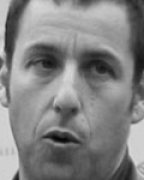
\includegraphics[width=0.1\textwidth]{images/intro/class0_0} &
		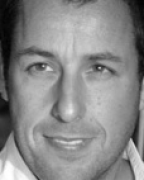
\includegraphics[width=0.1\textwidth]{images/intro/class0_1} & 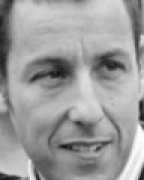
\includegraphics[width=0.1\textwidth]{images/intro/class0_2} & 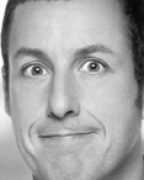
\includegraphics[width=0.1\textwidth]{images/intro/class0_3} & $\cdots$ \\ \hline
		Emma Watson & 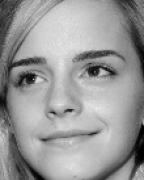
\includegraphics[width=0.1\textwidth]{images/intro/class1_0} &
		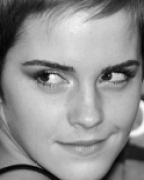
\includegraphics[width=0.1\textwidth]{images/intro/class1_1} & 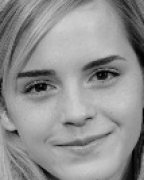
\includegraphics[width=0.1\textwidth]{images/intro/class1_2} & 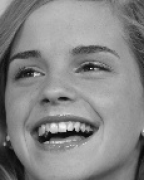
\includegraphics[width=0.1\textwidth]{images/intro/class1_3} & $\cdots$ \\ \hline
		Natalie Portman & 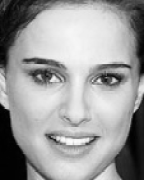
\includegraphics[width=0.1\textwidth]{images/intro/class2_0} & 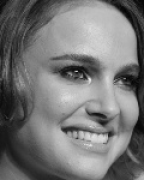
\includegraphics[width=0.1\textwidth]{images/intro/class2_1} & 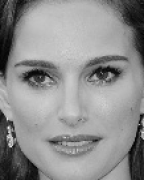
\includegraphics[width=0.1\textwidth]{images/intro/class2_2} & 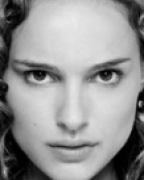
\includegraphics[width=0.1\textwidth]{images/intro/class2_3} & $\cdots$ \\ \hline
		$\qquad\qquad\vdots$ & $\qquad\vdots$ & $\qquad\vdots$ & $\qquad\vdots$ & $\qquad\vdots$ & $\ddots$ \\
	\end{tabular}
	\caption{Visualisierng einer Datenbank von Bildern von Gesichtern.}
	\label{fig:database}
\end{figure}
Aus dieser Datenbank \glqq{}lernt\grqq{} das Programm, neue Bilder zu klassifizieren, also den Personen aus der Datenbank zuzuordnen.
Das Wort \glqq{}neu\grqq{} bedeutet hier, dass dieses Bild nicht notwendigerweise in der Datenbank enthalten ist.
Die Person auf dem Bild muss aber in der Datenbank sein!
Würde die Datenbank in Abbildung~\ref{fig:database} wirklich nur diese drei Personen enthalten, so könnte man zum Beispiel kein Bild von Brad Pitt korrekt klassifizieren, auch wenn eine noch so gute Methode verwendet wird.
Die Datenbank und die Methode der Gesichtserkennung sind unabhängig voneinander.
Das heisst einerseits, aus der selben Datenbank können verschiedene Methoden lernen.
Andererseits kann ein und die selbe Methode verschiedene Datenbanken nutzen.
Wie gut die Gesichtserkennung am Schluss funktioniert hängt nicht nur von der Methode selbst ab, sondern auch von der Datenbank, welche diese verwendet.
Grundsätzlich gilt, dass jede Methode umso besser funktioniert, je mehr Bilder pro Person in der Datenbank gespeichert sind, die sie verwendet.
Mit \glqq{}gut funktionieren\grqq{} ist gemeint, dass neue Bilder mit hoher Wahrscheinlichkeit richtig klassifiziert werden.

Die in Abbildung~\ref{fig:database} gezeigten Bilder stammen aus einer Datenbank von über 10'000 Bildern von über 100 berühmten Persönlichkeiten \cite{Chen14}.
Die Bilder sind alle schwarz-weiss und zeigen lediglich die Gesichter der Personen.
Genau diese Datenbank werden wir auch für alle nachfolgenden Kapitel verwenden \textcolor{green}{(Link zur Datenbank folgt)}.
Allerdings kann auch eine andere Datenbank verwendet werden, sofern sie in das richtige Format gebracht wird \textcolor{green}{(Kapitel dazu folgt)}.

Das Grundgerüst eines Programms zur Gesichtserkennung in Python steht uns schon zur Verfügung.
Wir werden dieses in den folgenden Kapiteln zu einem voll funktionsfähigen Programm erweitern.
Der gesamte Code befindet sich im Anhang \textcolor{green}{(folgt)} und kann unter folgendem Link heruntergeladen werden \textcolor{green}{(Link zum Code folgt)}.
\section{Eigengesichter}
In diesem Kapitel werden wir sehen was die Eigengesichter eigentlich sind.
Zu einer gegebenen Datenbank werden wir diese berechnen und mit unserem Python Code visualisieren.
Allerdings werden wir noch noch keine Gesichtserkennung vornehmen.
\begin{tcolorbox}
	\centerline{\textbf{Lernziele Kapitel 1}}
	\begin{enumerate}[leftmargin=*]
		\item Darstellung eines schwarz-weiss Bildes als Vektor \textit{verstehen}.
		\item Die Begriffe Durchschnittsgesicht, Differenzgesicht und Eigengesicht \textit{verstehen}.
		\item Die Singulärwertzerlegung als Blackbox \textit{anwenden} können.
	\end{enumerate}
\end{tcolorbox}
\section{Vom Bild zum Vektor} \label{sec:vectormatrix}
\begin{tcolorbox}
	\centerline{\textbf{Lernziele Kapitel~\ref{sec:vectormatrix}}}
	\begin{enumerate}[leftmargin=*]
		\item Darstellung eines schwarz-weiss Bildes als Vektor \textit{verstehen}.
		\item Die grundlegenden Matrix und Vektor Operation in Python \textit{anwenden} können (Addition, Multiplikation, Einträge auslesen oder verändern).
	\end{enumerate}
\end{tcolorbox}
Der erste Schritt besteht darin, Bilder als Vektoren aufzufassen.
Das hat zwei Gründe: Erstens können wir diese nur so geeignet in Python darstellen und manipulieren.
Zweitens erlaubt uns das, Bilder in den Kontext der linearen Algebra zu bringen um deren mächtige Methoden anzuwenden.
Als Beispiel betrachten wir ein Bild der Auflösung $N=144$ Pixel (Breite) mal $M=180$ Pixel (Höhe), wie in Abbildung~\ref{fig:image_to_vector}.
Jedem Pixel wird nun eine reelle Zahl zwischen Null und Eins zugeordnet.
Nehmen wir das Pixel an der Stelle $\left(i,j\right)\in\mathbb N^M\times\mathbb N^N$.
Zum Beispiel entspricht $\left(1,N\right)$ dem Pixel in der oberen rechten Ecke des Bildes.
Diesem Pixel wird also eine Zahl $p_{ij}\in\left[0,1\right]$ zugeordnet.
Dabei bedeutet $p_{ij}=0$, dass das Pixel schwarz ist und $p_{ij}=1$, dass es weiss ist.
Die Zahlen dazwischen entsprechen den Graustufen.
Das gibt uns eine $N\times M$-Matrix deren Einträge gerade die $p_{ij}$ sind.
So können wir also ein schwarz-weiss Bild als Matrix auffassen.
Nun schreiben wir die Spalten dieser Matrix in einen Vektor wie in Abbildung~\ref{fig:image_to_vector} gezeigt.
Mit dieser Abbildungsvorschrift können wir jedem schwarz-weiss Bild der Auflösung $N\times M$ auf eindeutige Weise einen Vektor in $\left[0,1\right]^{N\cdot M}$ zuordnen.
Jeder solche Vektor lässt sich auch wieder als Bild darstellen.
Für diesen Schritt ist es egal ob das Bild ein Gesicht zeigt oder etwas anderes.
\begin{figure}[ht]
	\centering
	\begin{tabular}{m{3.5cm} m{1cm} c m{1cm} c}
		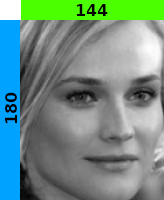
\includegraphics[width=0.2\textwidth]{images/vectormatrix/ImageToVector} &
		$\longrightarrow$ &
		$\begin{pmatrix}
			\textcolor{violet}{p_{11}} & \textcolor{orange}{p_{12}} & \cdots & \textcolor{olive}{p_{1N}} \\
			\textcolor{violet}{\vdots} & \textcolor{orange}{\vdots} & \ddots & \textcolor{olive}{\vdots} \\
			\textcolor{violet}{p_{M1}} & \textcolor{orange}{p_{M2}} & \cdots &  \textcolor{olive}{p_{MN}} \\
		\end{pmatrix}$ &
		$\longrightarrow$ &
		$\begin{pmatrix}
			\textcolor{violet}{p_{11}} \\
			\textcolor{violet}{\vdots} \\
			\textcolor{violet}{p_{M1}} \\
			\textcolor{orange}{p_{12}} \\
			\textcolor{orange}{\vdots} \\
			\textcolor{orange}{p_{M2}} \\
			\vdots \\
			\textcolor{olive}{p_{1N}} \\
			\textcolor{olive}{\vdots} \\
			\textcolor{olive}{p_{MN}} \\
		\end{pmatrix}$
	\end{tabular}
	\caption{Ein schwarz-weiss Bild kann als Matrix oder Vektor aufgefasst werden.}
	\label{fig:image_to_vector}
\end{figure}
\pagebreak[4]
\begin{aufgabe}
	Man betrachte das schwarz-weiss Bild, welches durch folgende Matrix beschrieben ist.
	\begin{equation*}
		\begin{pmatrix}
			1 & \frac{1}{4} \\
			\frac{1}{2} & 0 \\
			0 & \frac{3}{4} \\
		\end{pmatrix}
	\end{equation*}
	\begin{enumerate}[label=(\alph*)]
		\item Welche Werte für $N$ und $M$ beschreiben die Auflösung dieses Bildes?
		\item Wie sieht der Vektor aus, der dieses Bild beschreibt?
		\item Welches der folgenden drei Bilder entspricht dieser Matrix?
		
		\definecolor{onefourth}{rgb}{0.25, 0.25, 0.25}
		\definecolor{onehalf}{rgb}{0.5, 0.5, 0.5}
		\definecolor{threefourth}{rgb}{0.75, 0.75, 0.75}
		
		\qquad\qquad
		\begin{tikzpicture}
			\draw[step=1cm,white,very thin] (0,0) grid (2,3);
			\fill[white] (0,0) rectangle (1,1);
			\fill[onefourth] (1,0) rectangle (2,1);
			\fill[onehalf] (0,1) rectangle (1,2);
			\fill[white] (1,1) rectangle (2,2);
			\fill[black] (0,2) rectangle (1,3);
			\fill[threefourth] (1,2) rectangle (2,3);
		\end{tikzpicture}
		\qquad\qquad
		\begin{tikzpicture}
			\draw[step=1cm,white,very thin] (0,0) grid (2,3);
			\fill[black] (0,0) rectangle (1,1);
			\fill[threefourth] (1,0) rectangle (2,1);
			\fill[onehalf] (0,1) rectangle (1,2);
			\fill[black] (1,1) rectangle (2,2);
			\fill[white] (0,2) rectangle (1,3);
			\fill[onefourth] (1,2) rectangle (2,3);
		\end{tikzpicture}
		\qquad\qquad
		\begin{tikzpicture}
			\draw[step=1cm,white,very thin] (0,0) grid (2,3);
			\fill[black] (0,0) rectangle (1,1);
			\fill[onefourth] (1,0) rectangle (2,1);
			\fill[onehalf] (0,1) rectangle (1,2);
			\fill[black] (1,1) rectangle (2,2);
			\fill[white] (0,2) rectangle (1,3);
			\fill[threefourth] (1,2) rectangle (2,3);
		\end{tikzpicture}
	\end{enumerate}
\end{aufgabe}
\begin{losung*}
	Die Lösung der ersten beiden Teilaufgaben kann von Abbildung~\ref{fig:image_to_vector} abgelesen werden.
	Für die letzte Teilaufgabe erinnern wir uns, dass die Zahlen in $\left[0,1\right]$ fliessend den Graustufen von Schwarz (Null) bis Weiss (Eins) entsprechen.
	\begin{enumerate}[label=(\alph*)]
		\item Die Auflösung ist $N=3$ mal $M=2$ Pixel.
		\item Der Vektor ist gegeben durch
		\begin{equation*}
			\begin{pmatrix}
				1 \\
				\frac{1}{2} \\
				0 \\
				\frac{1}{4} \\
				0 \\
				\frac{3}{4} \\
			\end{pmatrix}.
		\end{equation*}
		\item Das mittlere Bild entspricht der Matrix.
	\end{enumerate}
\end{losung*}
In unserem Python Code ist die Funktion, welche eine $N\times M$ Matrix auf diese Weise in einen Vektor der Länge $N\cdot M$ überführt, bereits implementiert.
Sie befindet sich im File \texttt{eigenfaces.py} und heisst \texttt{matrix\_to\_vector}.
Wir betrachten diese nun etwas genauer, um die Manipulation von Matrizen und Vektoren in Python zu lernen.
\begin{lstlisting}[style=python]
import numpy as np

def matrix_to_vector(P, M, N):
	v = np.zeros(M * N)
	for i in range(M):
		for j in range(N):
			v[j + N * i] = P[i, j]
	return v
\end{lstlisting}
Das Argument \texttt{P} ist eine  \texttt{M} mal \texttt{N} Matrix und besteht aus den Einträgen $p_{ij}\in\left[0,1\right]$ wie oben.
Auf die Einträge von Vektoren und Matrizen kann über die eckigen Klammern $[$ und $]$ zugegriffen werden.
Wir brauchen aber auch die Umkehrung dieser Operation.
Das ist der Zweck folgender Übung.
\begin{aufgabe}
	Ergänzen Sie im File \texttt{eigenfaces.py} die Funktion \texttt{vector\_to\_matrix(v, M, N)}.
	Dabei ist \texttt{v} ein Vektor der Länge $\texttt{M}\cdot\texttt{N}$ wie oben.
	Die Funktion soll die zu \texttt{v} gehörende Matrix zurück geben.
	Sie können die ihre Lösung überprüfen indem Sie das Skript \texttt{vector\_to\_matrix\_test.py} laufen lassen.
\end{aufgabe}
\begin{losung*}
	Bei einer richtigen Lösung sollte das Skript \texttt{vector\_to\_matrix\_test.py} das Foto aus Abbildung~\ref{fig:image_to_vector} generieren.
	Die Lösung könnte zum Beispiel so aussehen:
\begin{lstlisting}[style=python]
import numpy as np

def vector_to_matrix(v, M, N):
	P = np.zeros(M, N)
	for i in range(M):
		for j in range(N):
			P[i, j] = v[j + N * i]
	return P
\end{lstlisting}
\end{losung*}
\nocite{*}
\bibliographystyle{plain}
\bibliography{references}
\end{document}